\chapter{Approximation Algorithms}
An algorithm for an optimization problem that yields a ``nearly''
optimal solution is called an approximation algorithm.
$0<C_{n}*$ cost of an optimal solution for an input of size
$n$ (e.g. length of a shortest path). $0<C_{n}$ cost of a solution
produced by an approximation algorithm. If 
$max(\frac{C_{n}}{C_{n}*},\frac{C_{n}*}{C_{n}})=\rho (n)$ then
the algorithm has an approximation ratio of $\rho (n)$.\\
(Remark: $\rho (n) \ge 1$)\\
$\rho (n) = 1$: optimal, $\rho(n) >> 1$: bad approximation\\
Trade-off: Cost of the approximation algorithm vs. quality of approximation.\\
An approximation scheme for an approximation problem is an 
algorithm with 2 inputs: $Problem + \epsilon>0$ such that
the algorithm is a $(1 + \epsilon)$ - approximation algorithm.\\
The approximation scheme is a polynomial time approximation
scheme if for each $\epsilon > 0$ the induced algorithm runs in polynomial time in $n$.
It is fully polynomial if it is polynomial in $n$ and in $1/\epsilon$.
\begin{example}
$O(n^(\frac{2}{3}))$, if $\epsilon' = \frac{3}{4}$ $O(n^(\frac{8}{\epsilon}))$ cost, i.e.
the costs are rising but not by a constant factor.
\end{example}
\begin{example}
$O((1/\epsilon)^2 * n^3)$ fully polynomial. $\epsilon = \frac{\epsilon}{4}
O(16*(\frac{1}{\epsilon}^2 * n^3))$.
\end{example}
\section{Heuristic Approaches}
\emph{Vertex Cover}: Given an undirected graph $G=(V,E)$ without parallel edges and without loops,
we look for a minimal set $V'$ of nodes such that each edge has at least one endpoint in $V'$.
\begin{example*}
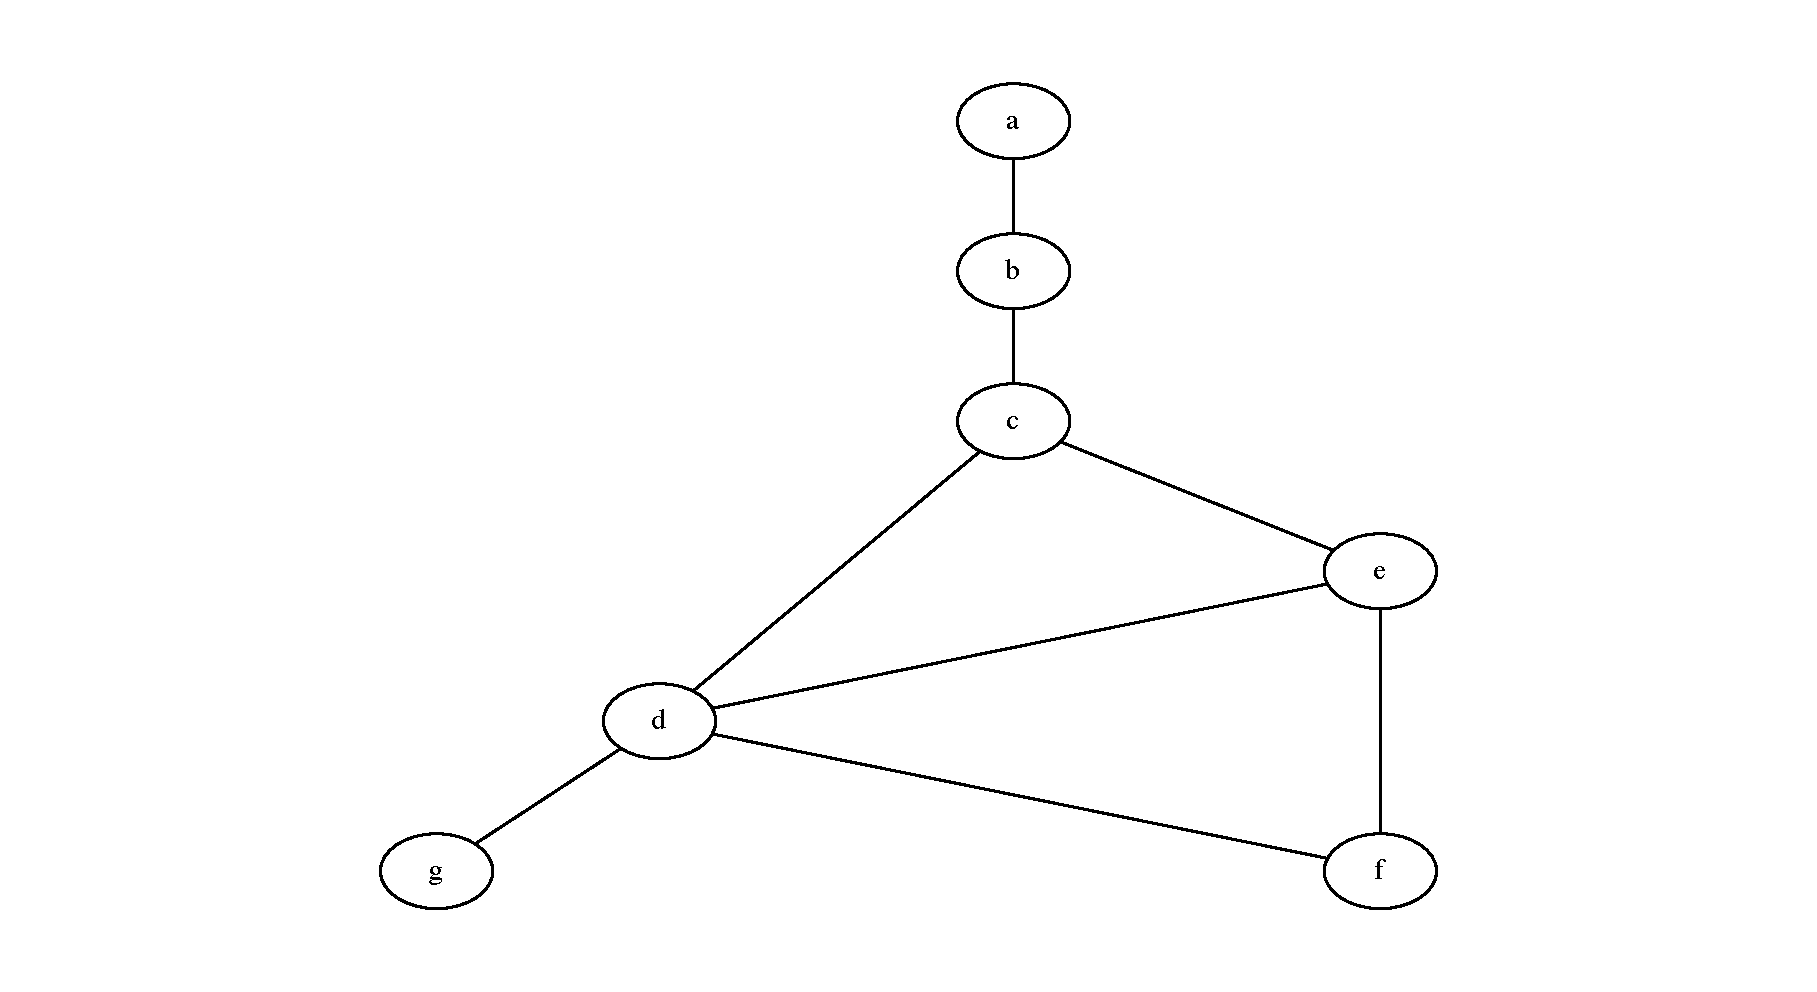
\includegraphics[width=\textwidth]{diagrams/Chapter7_Example1.pdf}
\end{example*}
\begin{algorithm}
\begin{algorithmic}[1]
\State $C \gets \emptyset$
\State $E' \gets E$
\While{$E' \neq \emptyset$}
	\State Choose an edge $\{u,v\}$ in $E'$.
	\State $C \gets C \cup \{u,v\}$
	\State Remove all edges from $E'$ with the end point $u$ or $v$.
\EndWhile
\end{algorithmic}
\caption{APPROX-VERTEX-COVER($G=(V,E)$)}
\end{algorithm}


\section{Probabilistic Analysis and randomized algorithms}

\textbf{Assistant search}
\begin{enumerate}
  \item[1] best = 0
  \item[2] for i = 1 .... n do\\
\noindent\hspace*{10mm}	interview candidate i\\
\noindent\hspace*{10mm}	if candidat i is better than best\\
\noindent\hspace*{20mm}		then best:= i\\
\noindent\hspace*{20mm}		employ candidate i (fire previous candidate)\\
\end{enumerate}

\underline{Analysis} of the cost that arise from interviews and hiring.\\
cost of an interview $c{_I}(low)$\\
cost of hiring: $c{_E}(high)$\\
Cost that arise in the worst case $O(n* c{_I} +  m * c{_E}$ ) if m people are hired 
and \\
$O(n * c{_I} +  n *  c{_E} )$ if n people are hired \\
worst case: if candidates show up in the order: worst first, \ldots best last

